% ==============================================================================
% LAB 119
% UNDERSÖKNING AV RC-KRETS
% ------------------------
%
% Author:
% Jonas Sjöberg     <tel12jsg@student.hig.se>
% Oscar Wallberg    <tco13owg@student.hig.se>
%
% License:
% Creative Commons Attribution-NonCommercial-ShareAlike 4.0 International
% See LICENSE.md for full licensing information.
% ==============================================================================

\section{Uppmätning av Bode-diagram}\label{bode}

\subsection{Experimentuppställning}\label{}
% ------------------------------------------------------------------------------
En så kallad experimentplatta eller "breadboard" används för att konstruera
kretsen som illustreras i Figur \ref{fig:rc-schema}.
\par För att generera en sinusformad signal används signalgeneratorn \texttt{HP33120A},
vars utgång kopplas genom en BNC-förgrening till oscilloskopet \texttt{Agilent 54621A}
och genom en BNC- banankontaktadapter, med ``banankablar'' till
breadboardplattans skruvterminaler.
\par Oscilloskopets första kanal visar signalen från kretsens ingång, punkten
\texttt{Vout} i \ref{fig:rc-schema}. Samma punkt utgör signalgeneratorns
utgång och vid några mätningar användes en T-koppling av BNC-kablar för att 
mata signalgeneratorns utgång till både experimentkopplingen och oscilloskopet.
En oscilloskopprob är ansluten till oscilloskopets andra kanal. Proben kopplas
till kretsens utgång, punkten \texttt{Vout} i \ref{fig:rc-schema} med en
oscilloskop-prob. Proben ställs till att dämpa med en faktor av 10:1 och den
vertikala skalan justeras en dekad
nedåt, så att båda kanalerna visas med samma skalfaktor.


\begin{figure}
    \centering
    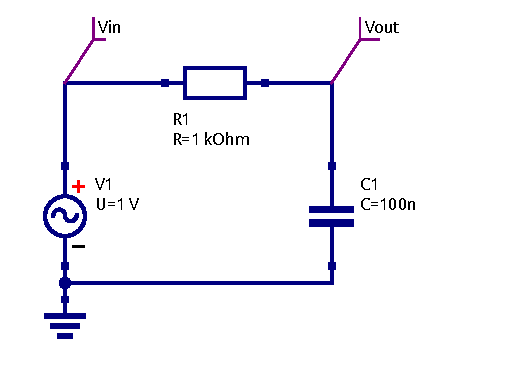
\includegraphics[width=0.8\linewidth]{sim/ee466_lab-4_prj/uppgift-0_schema}
    \caption[Schematisk ritning av labbkoppling, första ordningens RC-filter.]
    {Schematisk ritning av labbkoppling, första ordningens RC-filter.}
    \label{fig:rc-schema}
\end{figure}


\subsection{Mätresultat}\label{}
% ------------------------------------------------------------------------------
% TODO:

\subsection{Simulering}\label{}
% ------------------------------------------------------------------------------
Kretsen simuleras i \texttt{Qucs} enligt Figur~\ref{fig:bode-sim-ac},
Figur~\ref{fig:bode-sim-tran} och Figur~\ref{fig:bode-sim-param}.

\begin{figure}
    \centering
    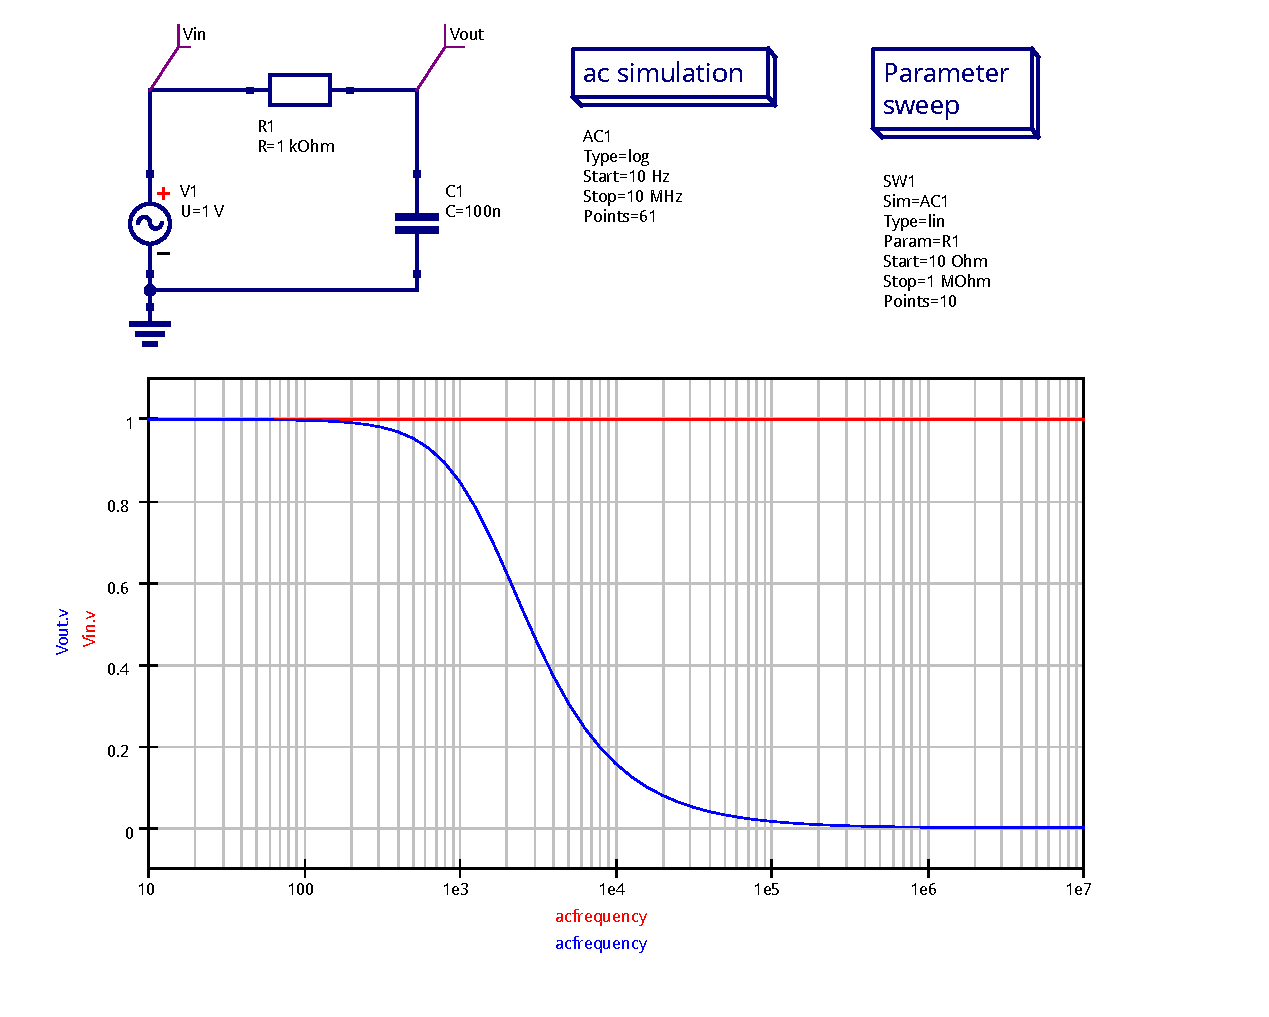
\includegraphics[width=\linewidth]{sim/ee466_lab-4_prj/uppgift-1_ac}
    \caption[] {Simulering av kretsens frekvensåtergivning.}
    \label{fig:bode-sim-ac}
\end{figure}

\begin{figure}[ht]
    \centering
    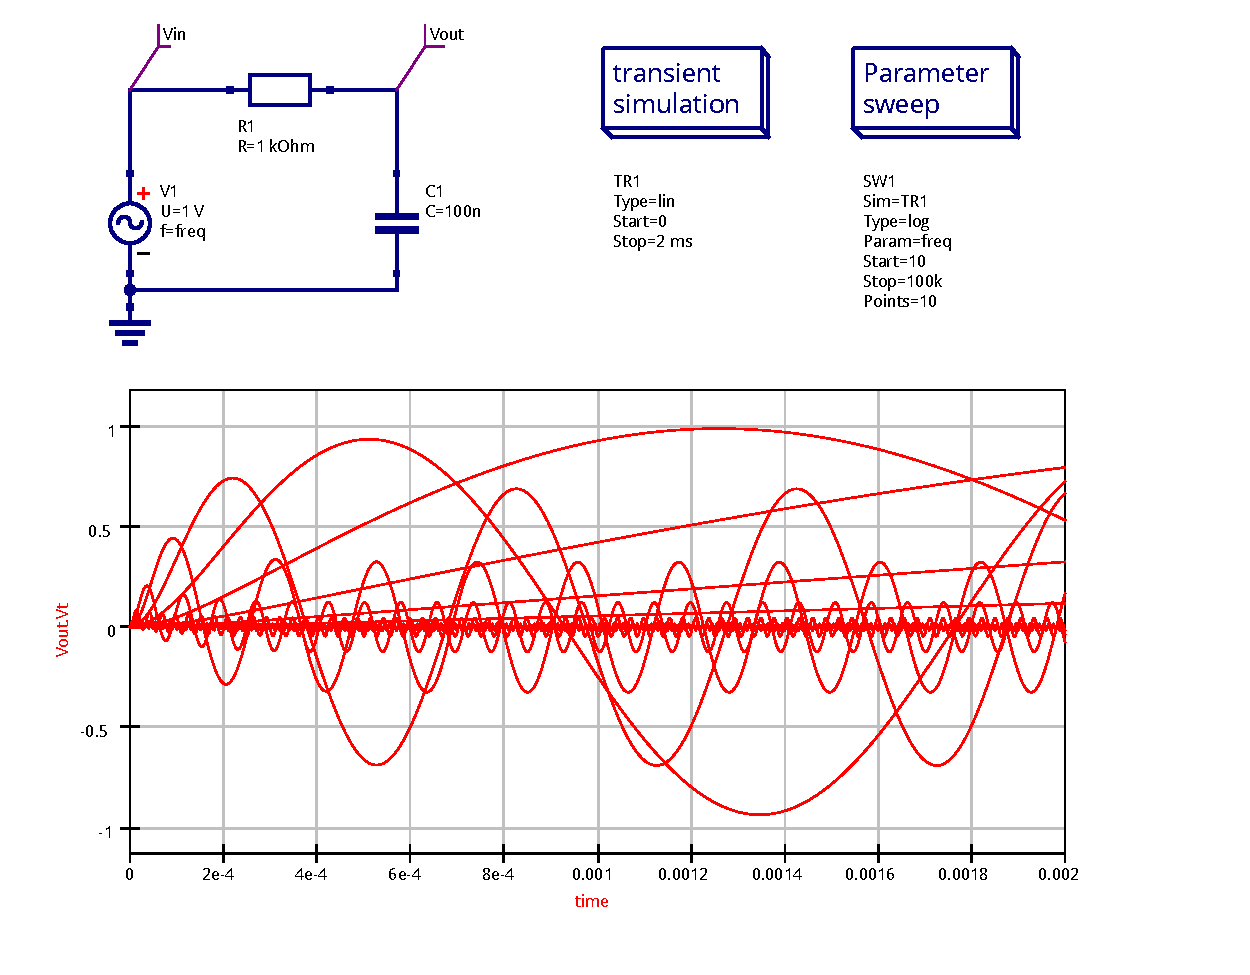
\includegraphics[width=\linewidth]{sim/ee466_lab-4_prj/uppgift-1_tran}
    \caption[] {Simulering av kretsen i tidsdomänen för olika frekvenser av $V_1$.}
    \label{fig:bode-sim-tran}
\end{figure}

\begin{figure}[ht]
    \centering
    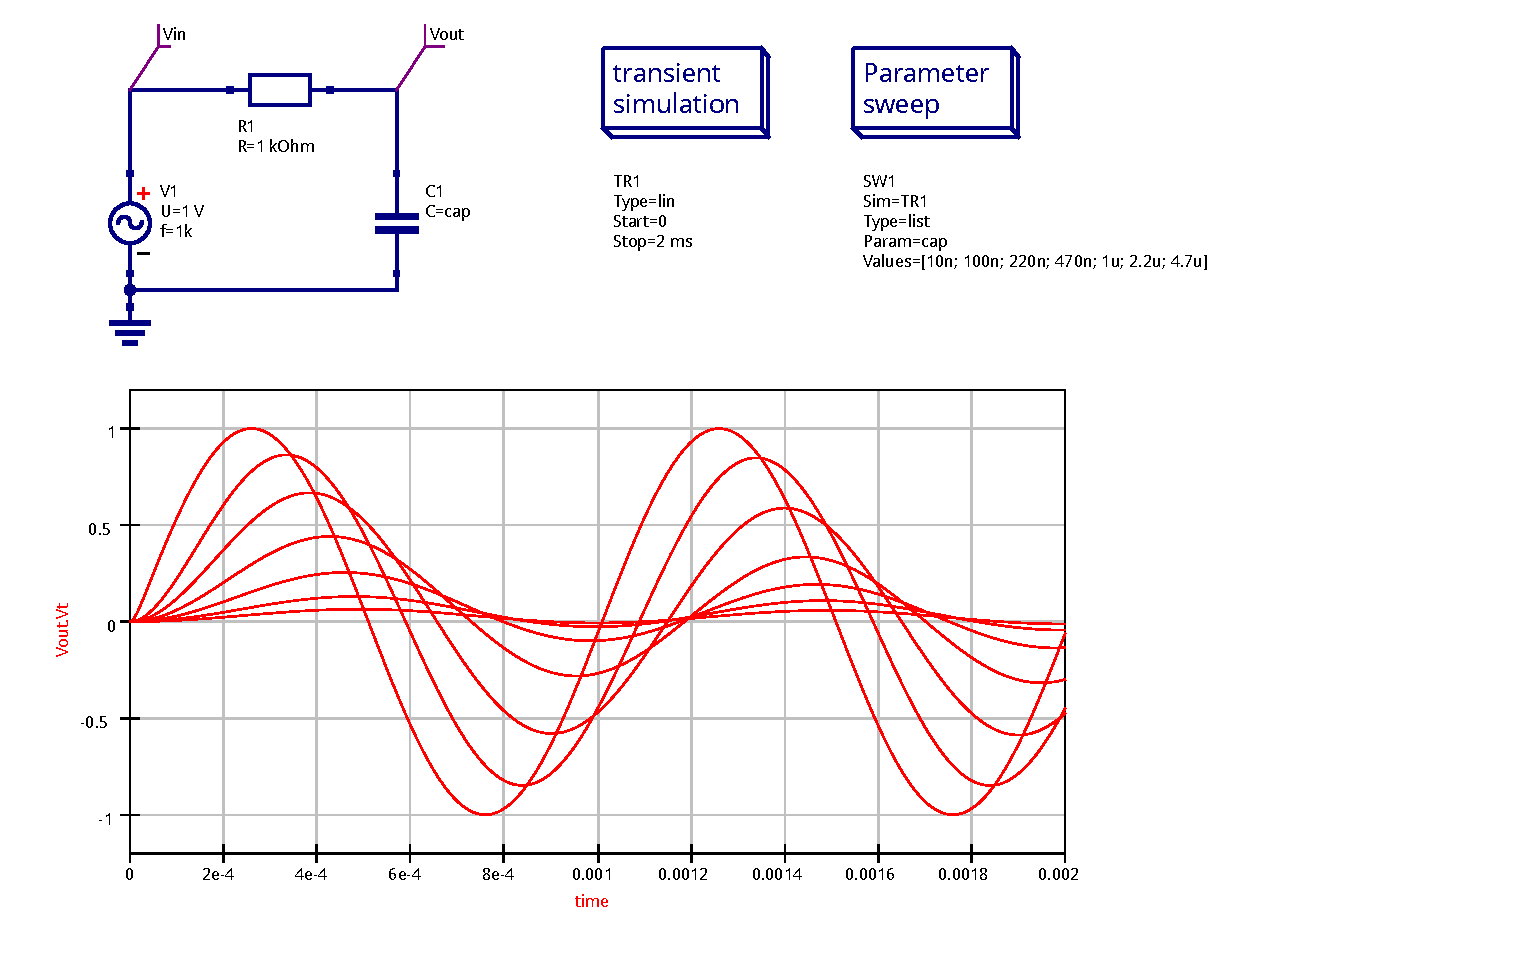
\includegraphics[width=\linewidth]{sim/ee466_lab-4_prj/uppgift-1_param}
    \caption[] {Simulering av kretsen i tidsdomänen för olika värden av $C_1$.}
    \label{fig:bode-sim-param}
\end{figure}


\subsection{Kommentar}\label{}
% ------------------------------------------------------------------------------
% TODO:


